% helix_geometry.tex — 圆柱螺旋几何示意图（TikZ standalone）
\documentclass[tikz,border=8pt]{standalone}
\usepackage{tikz}
\usetikzlibrary{3d,arrows.meta}
\begin{document}
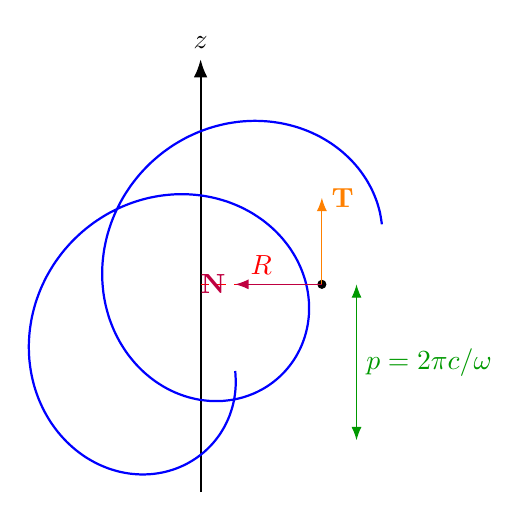
\begin{tikzpicture}[scale=1.1,>=Latex]
  % 螺旋轴
  \draw[thick,->] (0,-2.4) -- (0,2.6) node[above] {$z$};
  % 螺旋近似（折线模拟）
  \draw[thick,blue] plot[domain=0:720,samples=120,smooth]
    ({1.4*cos(\x)},{1.4*sin(\x)},{0.35*\x/57.2958-1.8});
  % 半径
  \draw[red,dashed] (0,0) -- (1.4,0) node[midway,above] {$R$};
  % 螺距标注
  \draw[<->,green!60!black] (1.8,-1.8) -- (1.8,0.0) node[midway,right] {$p=2\pi c/\omega$};
  % 局部标架示意
  \fill (1.4,0) circle (1.5pt);
  \draw[->,orange] (1.4,0) -- (1.4,1.0) node[right] {$\mathbf{T}$};
  \draw[->,purple] (1.4,0) -- (0.4,0) node[left] {$\mathbf{N}$};
\end{tikzpicture}
\end{document}
